\tikzset{%
  >=latex
}
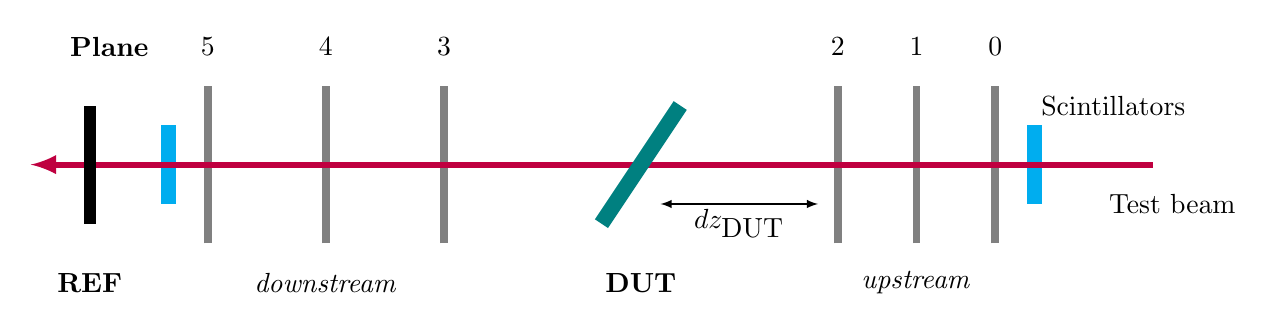
\begin{tikzpicture}
  \node at (-6.75,1.5) {\textbf{Plane}};
  % Scintillators (upstream)
  \draw [cyan, line width=0.2cm] (5, -0.5) -- (5, 0.5);
  \node at (6,.75) {Scintillators};
  % Scintillators (downstream)
  \draw [cyan, line width=0.2cm] (-6, -0.5) -- (-6, 0.5);
  % Plane 3-5
  \draw [gray, line width=0.1cm] (-2.5, -1) -- (-2.5, 1);
  \node at (-2.5,1.5) {3};
  \draw [gray, line width=0.1cm] (-4, -1) -- (-4, 1);
  \node at (-4,1.5) {4};
  \draw [gray, line width=0.1cm] (-5.5, -1) -- (-5.5, 1);
  \node at (-5.5,1.5) {5};
  \node at (-4,-1.5) {\emph{downstream}};
  % Plane 0-2
  \draw [gray, line width=0.1cm] (2.5, -1) -- (2.5, 1);
  \node at (2.5,1.5) {2};
  \draw [gray, line width=0.1cm] (3.5, -1) -- (3.5, 1);
  \node at (3.5,1.5) {1};
  \draw [gray, line width=0.1cm] (4.5, -1) -- (4.5, 1);
  \node at (4.5,1.5) {0};
  \node at (3.5,-1.5) {\emph{upstream}};
  % test beam
  \draw [purple, line width=0.075cm, ->] (6.5,0) -- (-7.75,0);
  \node at (6.75,-.5) {Test beam};
  % track
  %\draw [purple, line width=0.05cm] (5.5,0) -- (0.25,0.5);
  %\draw [purple, line width=0.05cm] (0.25,0.5) -- (-7,0);
  % DUT
  \draw [teal, line width=0.2cm] (-0.5, -0.75) -- (0.5, 0.75);
  \node at (0,-1.5) {\textbf{DUT}};
  \draw [black, <->] (0.25, -0.5) -- (2.25, -0.5);
  \node at (1.25,-0.75) {$dz_{\textrm{DUT}}$};
  % REF
  \draw [line width=0.15cm] (-7, -0.75) -- (-7, 0.75);
  \node at (-7,-1.5) {\textbf{REF}};
\end{tikzpicture}
